Die Breitensuche ist nicht nur ein Verfahren, um Knoten in einem Graphen systematisch aufzulisten. Dank der speziellen Reihenfolge, in der die Knoten besucht werden (zuerst die direkten Nachbarn, dann dessen Nachbarn und so weiter), sind wir sicher, dass wir jeden erreichbaren Knoten über einen kürzesten Pfad erreichen. In diesem Abschnitt werden wir den Algorithmus, den wir im vorherigen Abschnitt kennengelernt haben, so abändern und erweitern, dass wir zuerst den Abstand zwischen zwei Knoten in einem Graphen berechnen können und dann sogar die Knoten auf dem kürzesten Pfad auflisten.

\subsection{Die Länge des kürzesten Pfades}

Wie wir schon wissen, ist der \textbf{Abstand} zwischen zwei Knoten definiert als die Länge des kürzesten Pfades zwischen diesen zwei Knoten. Ein \textbf{Pfad} ist eine Folge von Knoten, die, wie eine Kette, eine Kante zum vorherigen und zum nächsten Knoten haben. Die \textbf{Länge} eines Pfades ist die Anzahl Kanten auf dem Pfad.

\begin{beispiel}
Betrachte folgenden Graphen.
\begin{figure}[H]
\centering
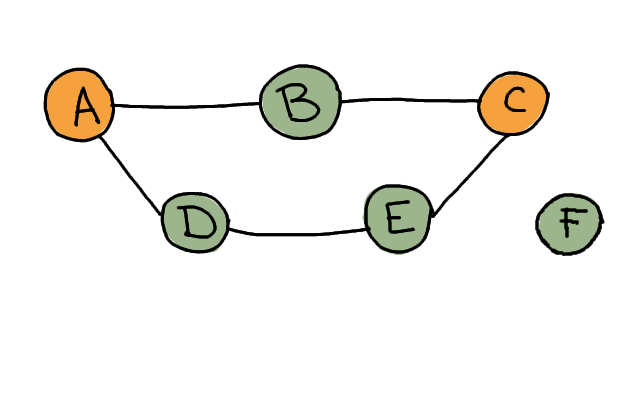
\includegraphics[width=0.5\linewidth]{Pictures/SP/abstand_def.png} 
\end{figure}
Der Abstand zwischen \textbf{A} und \textbf{C} ist \(2\). Zwischen \textbf{A} und \textbf{C} gibt es zwei Pfade: \textbf{ABC} und \textbf{ADEC}. Der Pfad \textbf{ABC} ist der kürzeste und hat zwei Kanten, somit ist der Abstand zwischen \textbf{A} und \textbf{C} \(2\).

Bevor du weiterliest, überlege kurz, was der Abstand zwischen \textbf{A} und \textbf{F} sein könnte.

Beobachte, dass es zwischen \textbf{A} und \textbf{F} gar keinen Pfad gibt. Sie sind nicht verbunden. In einem solchen Fall sagen wir, dass der Abstand \(\infty\) (unendlich) ist.
\end{beispiel}

\begin{aufgabe}\label{aufgabe_abstand_ex}
Betrachte folgenden Graphen.
\begin{figure}[H]
    \centering
    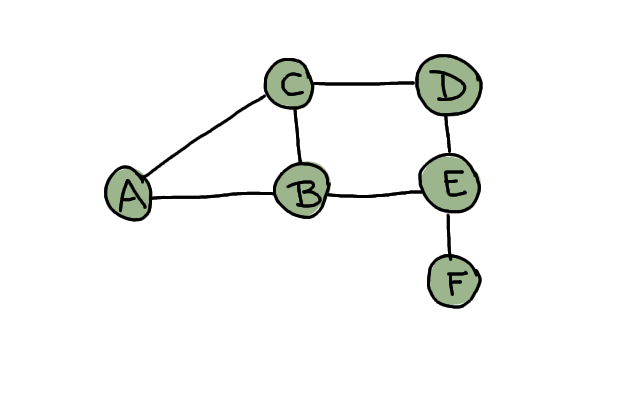
\includegraphics[width=0.5\textwidth]{Pictures/SP/abstand_ex.png} 
    \label{fig:abstand_ex}
\end{figure}
Was ist der Abstand zwischen \textbf{A} und \textbf{F}?
Was ist der Abstand zwischen \textbf{C} und \textbf{E}?
\end{aufgabe}
\begin{aufgabe}\label{aufgabe_abstand}
\begin{enumerate}[(a)]
\item \label{aufgabe_abstand_k5} Zeichne einen vollständigen Graphen mit 5 Knoten. Was ist die Länge des kürzesten Pfades zwischen zwei beliebigen Knoten?
\item \label{aufgabe_abstand_gitter23} Zeichne einen Gittergraphen mit 2 mal 3 Knoten. Welche zwei Knoten sind am weitesten auseinander? Bestimme den Abstand (die Länge des kürzesten Pfades) zwischen diesen zwei Knoten.
\item \label{aufgabe_abstand_kreis6} Zeichne einen Kreis mit 6 Knoten. Welche zwei Knoten sind am weitesten auseinander? Wie weit sind sie voneinander entfernt?
\end{enumerate}
\end{aufgabe}

\subsubsection*{Das Wikipedia-Spiel}
Als wir den Breitensuchealgorithmus in Worten definiert hatten, haben wir das Wikipedia-Spiel kennengelernt. Alice gibt Bob zwei Wikipediaartikel vor und er muss vom Startartikel aus auf Links klicken, bis er auf den Zielartikel stosst. Das Ziel ist mit möglichst wenigen Klicks auszukommen.

Der Wikipedia-Graph ist nicht so übersichtlich und regelmässig, wie die Graphen, die wir gerade gesehen haben. Um den kürzesten Pfad zwischen zwei Artikel zu finden, muss Bob systematisch vorgehen. 
\begin{figure}[H]
    \centering
    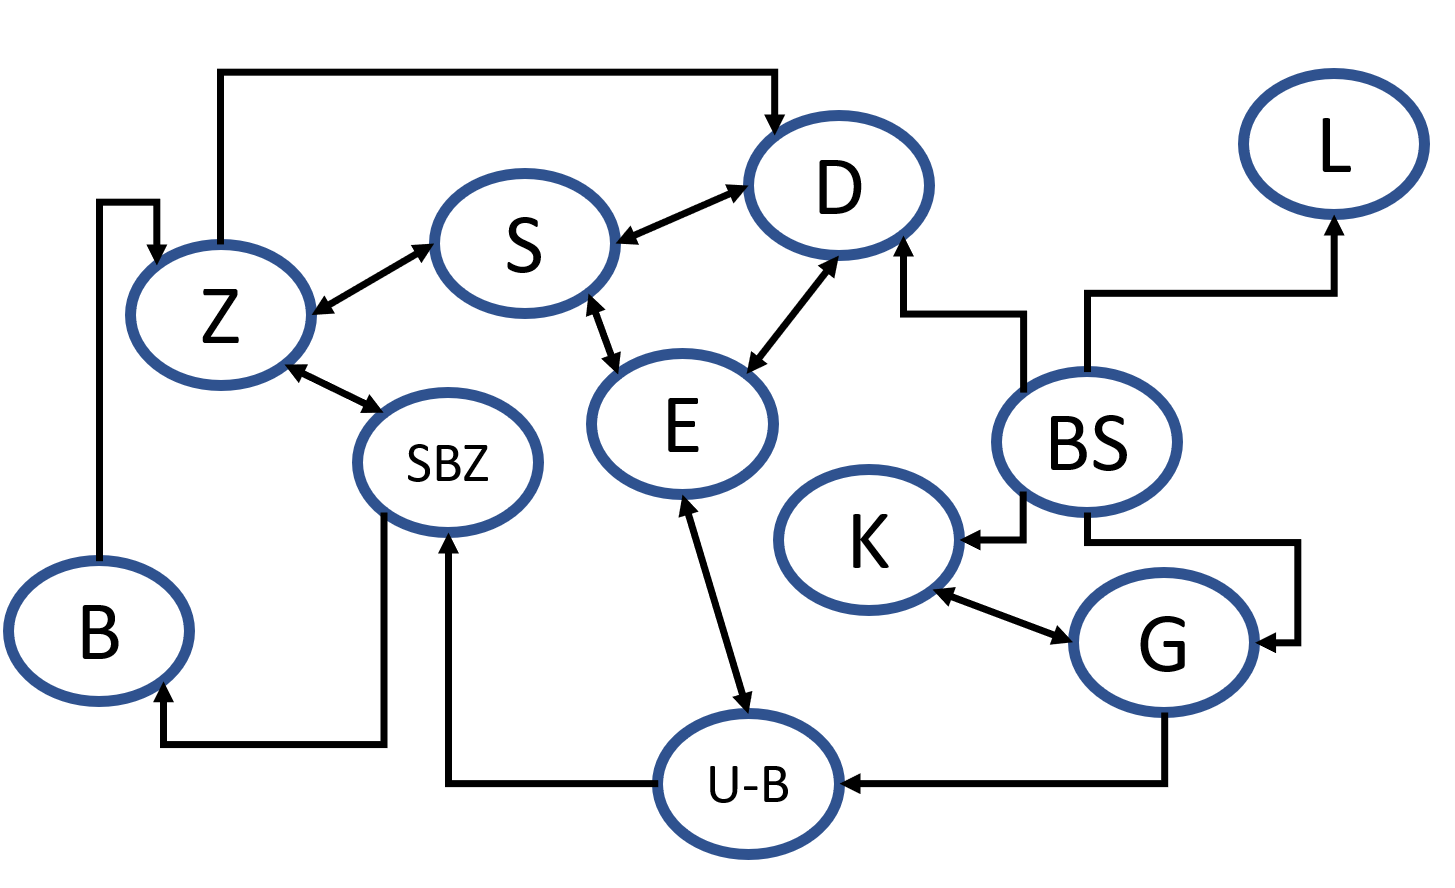
\includegraphics[width=0.7\textwidth]{Pictures/Wikipedia.PNG} 
    \caption{Die Verlinkung von Wikipedia-Artikeln als Graph.}
    \label{fig:wikipedia_graph}
\end{figure}

Wenn er nach dem Breitensuchealgorithmus vorgeht, wird er den Startartikel im Browser aufmachen (\textit{Breitensuche}, in unserem Beispiel von vorher) und dann jeden Link (\textit{Deutschland}, \textit{Graph}, \textit{Laufzeit}, \textit{Knoten}) in einem neuen Tab öffnen und anschliessend den Tab mit der Breitensuche schliessen. All die Artikel, die er jetzt im Browser offen hat, sind ein Klick vom Breitensucheartikel entfernt. Jetzt kann er dasselbe für den zuerst geöffneten noch offenen Tab (\textit{Deutschland}) tun. Er muss sich einfach merken, dass die neugeöffneten Tabs (\textit{Eisenbahn}, \textit{Schweiz}) sind jetzt 2 Klicks entfernt: Ein Klick mehr als die Seite, woher er kommt (\textit{Deutschland}). Er kann einfach für jeden Artikel aufschreiben, wie viele Klicks er vom Breitensucheartikel entfernt ist. Jeder nicht besuchte benachbarte Artikel wird ein Klick weiter sein.

\begin{aufgabe}\label{aufgabe_wikipedia_spiel}
Alice und Bob spielen das Wikipedia-Spiel auf den Graphen in Abbildung \ref{fig:wikipedia_graph}. Bob startet bei \textbf{BS} und muss in möglichst wenig Klicks \textbf{SBZ} erreichen. Helfe Bob herauszufinden, wie viele Klicks er braucht. Wie musst du den Breitensuchealgorithmus modifizieren, um die minimale Anzahl Klicks zu ermitteln? Führe deinen modifizierten Breitensuchealgorithmus auf diesen Graphen aus. Wie sehen in jedem Schritt \texttt{queue} und \texttt{visited} aus? Wo schreibst du die Abstände zwischen dem Startknoten und jedem besuchten Knoten auf?
\end{aufgabe}

\subsubsection*{Abstand zwischen zwei Knoten in Python ausrechnen}
Die Aufgabe \ref{aufgabe_wikipedia_spiel} hat mehrere möglichen Lösungen. Wir werden eine der Varianten in Python implementieren. In dieser Variante werden wir die Abstände genau dort speichern, wo wir sie brauchen: in der Warteschlange. Grundsätzlich gibt es zwei grosse Änderungen:
\begin{enumerate}
    \item Die Warteschlange enthält nicht nur Knoten, sondern auch deren Abstand vom Startknoten.
    \item Das Programm gibt anstatt von der Liste aller besuchten Knoten den Abstand zwischen Start- und Zielknoten zurück.
\end{enumerate}

\begin{figure}[H]
    \centering
    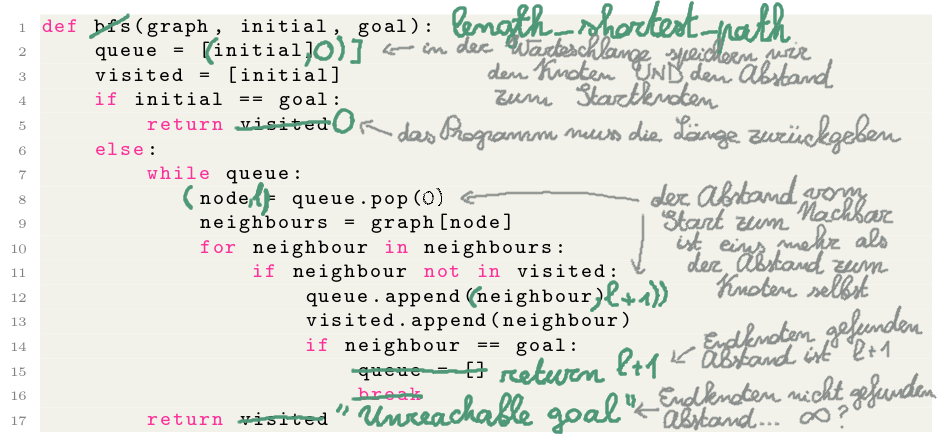
\includegraphics[width=\textwidth]{Pictures/SP/bfs_goal-to-length.png}
    \caption{Programm, das einen bestimmten Knoten sucht, in ein Programm umschreiben, das den Abstand zwischen Start- und Zielknoten findet.}
    \label{fig:bfs_goal_to_length}
\end{figure}

\begin{lstlisting}[language=Python, caption={Programm, das den Abstand zwischen \texttt{initial} und \texttt{goal} berechnet.}, label={lst:length_shortest_path}]
def length_shortest_path(graph, initial, goal):
    queue = [(initial, 0)]
    visited = [initial]
    if initial == goal:
        return 0
    else:
        while queue:
            (node, length) = queue.pop(0)
            new_length = length + 1
            neighbours = graph[node]
            for neighbour in neighbours:
                if neighbour not in visited:
                    queue.append((neighbour, new_length))
                    visited.append(neighbour)
                    if neighbour == goal:
                        return new_length
        return "There is no path between initial and goal in the given graph"
\end{lstlisting}

\begin{framed}
\paragraph{\textcolor{blue-violet}{Was haben wir gelernt:}}
Um die \textbf{Länge des kürzesten Pfades} zwischen Start- und Zielknoten in einem Graphen zu finden, können wir eine abgeänderte Version vom Breitensuchealgorithmus verwenden. Wie in der normalen Breitensuche, verwenden wir eine Warteschlange, um die zu besuchenden Knoten zu speichern. Aber in dieser Version enthält die Warteschlange nicht nur die zu besuchende Knoten, sondern auch deren \textbf{Abstand vom Startknoten}. Wir können diesen Abstand sehr einfach berechnen: Die Nachbarn eines Knotens sind \textbf{um \(1\) weiter}, als der Knoten selbst.

Wenn die Breitensuche abbricht, weil der Zielknoten gefunden wurde, dann können wir dessen Abstand aus der Warteschlange einfach ablesen. Die Breitensuche kann aber auch terminieren, ohne den Zielknoten gefunden zu haben. Wenn der Zielknoten im Graphen existiert, aber vom Startknoten nicht erreicht werden kann, dann sagen wir, dass der Start- und Zielknoten zu unterschiedlichen \textbf{Zusammenhangskomponenten} gehören.
\end{framed}


\subsubsection*{\textcolor{blue-violet}{Teste dich selber}}
\begin{aufgabe}\label{laenge_kontrollfragen}
Beantworte folgende Fragen.
\begin{enumerate}[(a)]
\item Wie definiert man den Abstand zwischen zwei Knoten in einem Graphen?
\item Was hat die Breitensuche mit dem Abstand zwischen zwei Knoten zu tun?
\item Gregory behauptet: ''Wenn die Breitensuche terminiert, ohne den Zielknoten gefunden zu haben, dann ist der Zielknoten nicht im Graphen enthalten''. Hat er recht? Begründe deine Antwort.
\item Welche zusätzliche Informationen müssen wir während der Breitensuche speichern, um die Länge des kürzesten Pfades zwischen Start- und Zielknoten berechnen zu können?
\end{enumerate}
\end{aufgabe}


\paragraph{Über wie vielen Ecken kennt jeder jeden?}
Alice hat gehört, dass jeder jeden im Schnitt über 6,6 Ecken kennt. Das heisst, jede zwei Menschen auf der Welt sind über höchstens 7 Kontaktpersonen bekannt. Alice ist von dieser Theorie sehr begeistert und möchte herausfinden, über wie vielen Ecken sie eine Person kennt, die schon Mal von einem Panda gebissen worden ist.

\begin{aufgabe}\label{aufgabe_panda_gebissen}
Hier ist eine Beschreibung von den Freundschaften von Alice und ihren Freunden.
\begin{displayquote}
Bob ist der beste Freund von Alice. Bob kennt ausserdem Charlie und David. Charlie, Elisabeth und Fred sind sehr eng befreundet und essen zusammen Kuchen jedes Wochenende. Fred und Alice kennen beide Gregory. Gregory und Hannah haben dieselbe Primarschule besucht und waren mit Jakob in einer Klasse. Jakob hat Fred im Militär kennengelernt. Jakob hat eine Schwester namens Lucy, und sie wurde einmal von einem Panda gebissen, als sie mit einer Bambushandtasche ins Zoo ging.
\end{displayquote}

\begin{enumerate}[(a)]
    \item Formalisiere die Freundschaften von Alice und ihrer Freunden als Graph. Was sind die Knoten? Wann sind zwei Knoten durch eine Kante verbunden? Ist der Graph gerichtet oder ungerichtet?
    \item Führe den modifizierten Breitensuchealgorithmus aus, um den Abstand im Freundschaftsgraphen zwischen Alice und Lucy zu bestimmen.
    \item Stelle den Freundschaftsgraphen in Python als Liste der Nachbarn dar.
    \item Führe das Programm \texttt{length\_shortest\_path} auf dem Freundschaftsgraphen aus. Wähle Start- und Zielknoten so, dass der Abstand im Graphen am grössten ist. Über wie vielen Ecken kennt jeder jeden in diesem Freundschaftsgraphen? 
\end{enumerate}

\end{aufgabe}

\paragraph{Norbert, der Staubsauger-Roboter}\label{norbert}
Norbert ist ein alter Staubsauger-Roboter. Er putzt das Zimmer den ganzen Tag und nun hat er fast kein Akku mehr.
\begin{wrapfigure}{l}{0.5\textwidth}
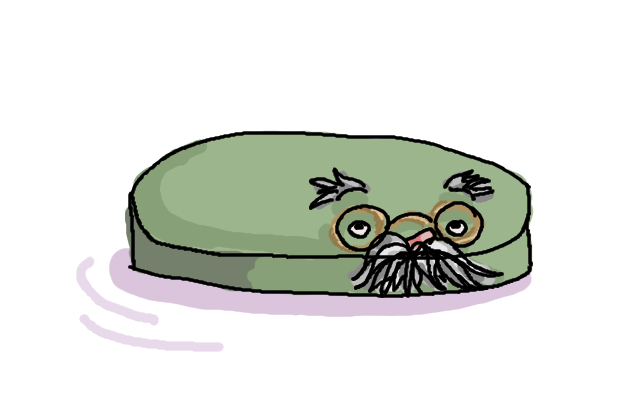
\includegraphics[width=0.9\linewidth]{Pictures/SP/norbert.png} 
\label{fig:norbert}
\end{wrapfigure}
Deswegen muss er so schnell wie möglich zurück zur Aufladestation.
Das Zimmer ist gefliest und Norbert kann von einer Fliese auf die andere fahren (das nennt er Schritt), aber nur nach vorne, nach hinten, nach links oder nach rechts, weil er sich nur um 90 Grad drehen kann. Ausserdem stehen im Zimmer Möbel herum, unter welchen Norbert nicht passt. Wie viele Schritte muss er bis zur Aufladestation fahren?

Norbert hat eine ziemlich gute mentale Karte vom Zimmer. Er weiss, dass das Zimmer 8 mal 6 Fliesen gross ist und einige grosse Schränke, Bücherregale und Sofas enthält. Er weiss genau, wo jedes Möbelstück steht.
\begin{figure}[H]
    \centering
    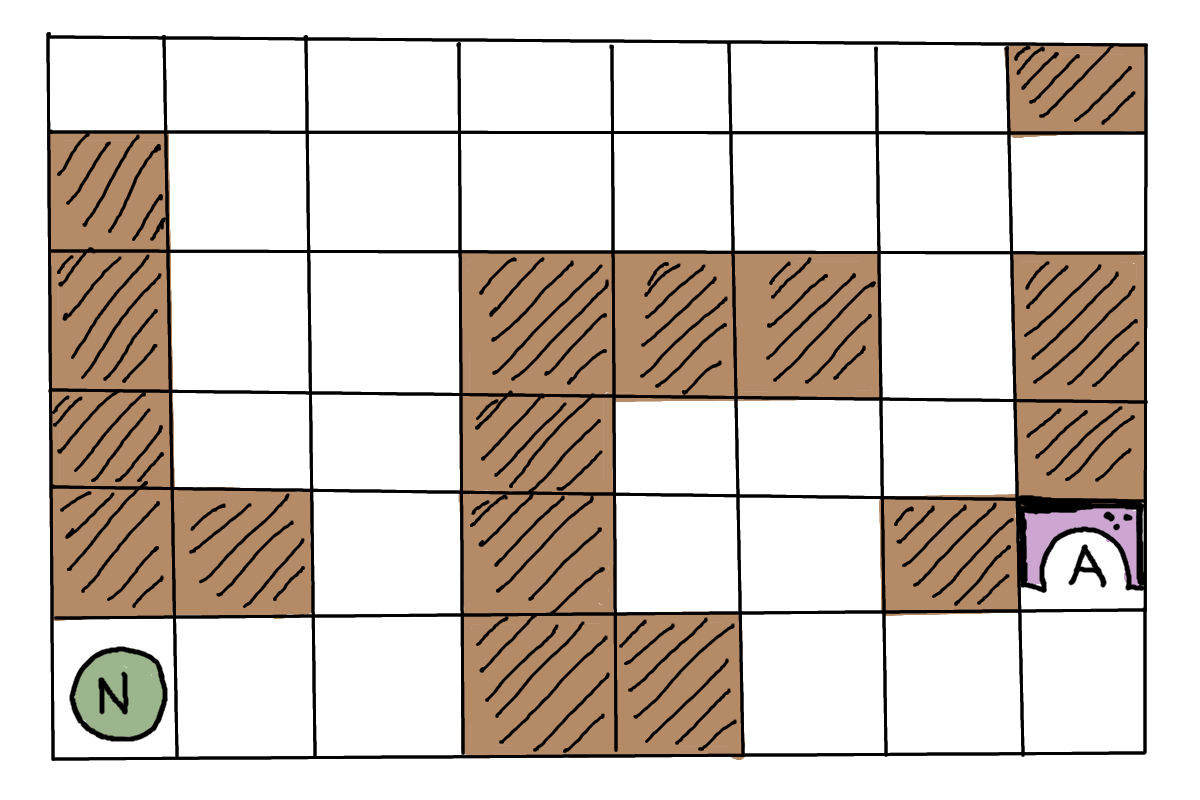
\includegraphics[width=\textwidth]{Pictures/SP/norbert_zimmer.png}
    \caption{Das Zimmer, wo sich Norbert befindet. In braun sind die Möbel markiert, unter welchen Norbert nicht passt. Norbert ist unten links, die Aufladestation ist unten rechts.}
    \label{fig:norbert_zimmer}
\end{figure}

\begin{aufgabe}\label{aufgabe_norbert}
\begin{enumerate}[(a)]
\item Modelliere das Problem von Norbert als Graph. Was sind die Knoten? Was sind die Kanten? Ist der Graph gerichtet? Wie modellierst du die Möbel?
\item Norbert hat nur noch Akku für 15 Schritte. Benutze den abgeänderten Breitensuchealgorithmus, um herauszufinden, ob er es noch schafft, die Aufladestation zu erreichen.
\item Wie viel Akku muss Norbert mindestens haben (gemessen in Schritte, die er noch machen kann), wenn er sicher sein will, dass er aus jeder Position im Zimmer die Aufladestation erreichen kann?
\item Schreibe den Graphen, den du aus Abbildung \ref{fig:norbert_zimmer} modelliert hast, in Python in der ''Liste der Nachbarn''-Darstellung.
\item Führe das Programm \texttt{length\_shortest\_path} aus, um die Länge des kürzesten Pfades zwischen Norbert und der Aufladestation zu bestimmen. Vergleiche das Ergebnis mit dem, was du in der Teilaufgabe (b) berechnet hast.
\end{enumerate}
\end{aufgabe}



\subsection{Der kürzeste Pfad}
Es ist sicher nützlich zu wissen, dass Bob in nur drei Klicks den Wikipedia-Artikel über den Zürcher Strassenbahnnetz erreichen kann, wenn der beim Breitensucheartikel startet; oder dass Alice über 3 Ecken jemanden kennt, der von einem Panda gebissen wurde; oder dass Norbert der Staubsauger-Roboter in 18 Schritten die Aufladestation erreichen kann. Aber wäre es nicht noch nützlicher zu wissen, welche Links Bob anklicken, oder welche Freunde und Freundesfreunde Alice kontaktieren, oder wo lang Norbert fahren müssen?

\subsubsection*{Norbert der Staubsauger-Roboter}
In einer Kontrollaufgabe haben wir Norbert den Staubsauger-Roboter kennengelernt. Der Boden des Zimmers, welches Norbert putzt, ist gefliest, und Norbert kann in einem ''Schritt'' von der Fliese, wo er ist, auf eine Fliese fahren, die sich vor ihm, hinter ihm, links von ihm oder rechts von ihm befindet. Aber es gibt Fliesen, auf welchen er nicht fahren kann, denn dort stehen Möbel (Schränke, Bücherregale, Sofas), unter welchen Norbert nicht passt. Norbert weiss genau, wo er sich befindet, wo die Aufladestation ist und wo all die Möbel stehen, die er umfahren muss.
\begin{figure}[H]
    \centering
    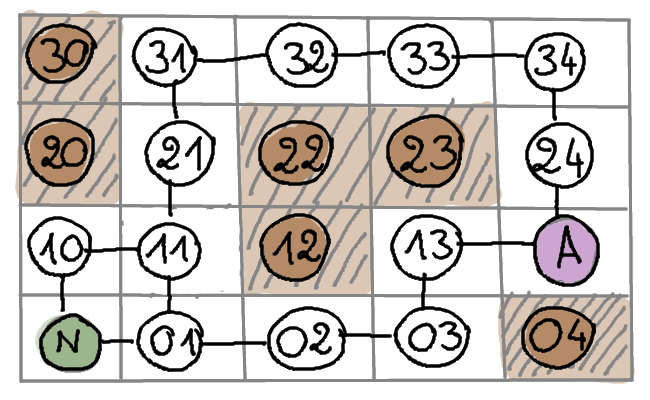
\includegraphics[width=0.6\textwidth]{Pictures/SP/norbert_klein_graph.png}
    \caption{Ein Zimmer für Norbert, schon als Graph modelliert. Die braunen isolierten Knoten stellen die Möbel dar.}
    \label{fig:norbert_klein_graph}
\end{figure}
Wir können das Zimmer als Graph modellieren, indem wir jeder Fliese einen Knoten zuordnen. Zwischen zwei Knoten gibt es eine Kante, wenn Norbert von der ersten entsprechenden Fliese auf die zweite in einem ''Schritt'' fahren kann.

Wir werden jetzt Norbert den Staubsauger-Roboter helfen, so schnell wie möglich seine Aufladestation zu erreichen. Wie auch für die Länge des kürzesten Pfades, gibt uns der Breitensuchealgorithmus alle benötigten Informationen, wir müssen sie nur speichern und richtig verwenden.

Nehmen wir an, wir führen jetzt die klassische Breitensuche aus. Wir fangen beim Startknoten \textbf{N} an und fügen dessen zwei Nachbarn \textbf{01} und \textbf{10} in die Warteschlange ein. Dann entfernen wir \textbf{01} aus der Warteschlange und fügen dessen Nachbarn hinzu: \textbf{02} und \textbf{11}. Dann entfernen wir \textbf{10}, welcher keine unbesuchten Nachbarn hat. Dann entfernen wir \textbf{02} und fügen \textbf{03} ein. Dann entfernen wir \textbf{11} und fügen \textbf{21} ein. Dann entfernen wir \textbf{03} und fügen \textbf{13} ein. Dann entfernen wir \textbf{21} und fügen \textbf{31} ein. Dann entfernen wir \textbf{13} und wir haben \textbf{A} schon gefunden. Die Knoten werden also in der folgenden Reihenfolge besucht.
\begin{lstlisting}[language=Python]
visited = ["N", "01", "10", "02", "11", "03", "21", "13", "31", "A"]
\end{lstlisting}
Aber wie können wir jetzt daraus den Pfad ausrechnen?


Die wichtige Beobachtung ist, dass wir \textbf{A} als Nachbar von \textbf{13} gefunden haben. Wir sagen dazu, dass \textbf{13} der \textbf{Elternknoten} von \textbf{A} ist. Das bedeutet, dass der kürzeste Pfad von \textbf{N} nach \textbf{A} über \textbf{13} verläuft.
\begin{figure}[H]
    \centering
    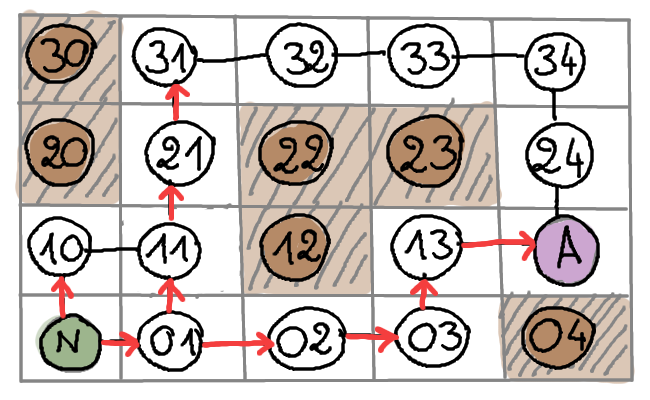
\includegraphics[width=0.6\textwidth]{Pictures/SP/norbert_klein_graph_arrows.png}
    \caption{Wir haben mit roten Pfeilen die Kanten markiert, welche wir bei der Breitensuche verwendet hatten. Um den kürzesten Pfad von \textbf{N} nach \textbf{A} zu finden, müssen wir nur die Pfeile von \textbf{A} nach \textbf{N} zurückverfolgen.}
    \label{fig:norbert_klein_graph_arrows}
\end{figure}
Wenn es einen kürzeren Pfad über einen anderen Knoten gegeben hätte, hätten wir \textbf{A} früher gefunden als Nachbar von einem anderen Knoten als \textbf{13}. Also muss \textbf{13} auf dem kürzesten Pfad liegen. Wir haben nun das Problem reduziert: Wir müssen nur noch den kürzesten Pfad zwischen \textbf{N} und \textbf{13} finden.

Wir gehen analog vor und fragen uns, woher wir \textbf{13} erreicht haben, das heisst wir suchen dessen Elternknoten. Den Knoten \textbf{13} haben wir als Nachbar von \textbf{03} gefunden. Dann muss \textbf{03} auch auf dem kürzesten Pfad liegen. Diese Kette lässt sich weiter führen: Den Knoten \textbf{03} haben wir von \textbf{02} aus gefunden, und \textbf{02} von \textbf{01} aus, und \textbf{01} von \textbf{N} aus. Der kürzeste Pfad ist somit:
\begin{lstlisting}
N - 01 - 02 - 03 - 13 - A.
\end{lstlisting}

Um den kürzesten Pfad aufzulisten, haben wir die roten Pfeilen aus Abbildung \ref{fig:norbert_klein_graph_arrows} zurückverfolgt, von \textbf{A} zurück nach \textbf{N}, in der umgekehrten Reihenfolge, in der die Breitensuche sie gefunden hatte. Diesen Verfahren nennt man \textbf{Backtracking}.

Aus einem Knoten können mehrere ''rote Pfeile'' ausgehen (weil ein Knoten mehrere Nachbarn haben kann, die wegen ihm in die Warteschlange eingefügt werden), aber maximal ein Pfeil kann darauf zeigen (weil wir Knoten, die wir schon gesehen haben, kein zweites Mal in die Warteschlange einfügen). Alle ''rote Pfeile'', wenn wir sie in die andere Richtung verfolgen, führen nach \textbf{N}, und zwar über den kürzesten Pfad.

\begin{aufgabe}\label{aufgabe_find_shortest_path}
Betrachte folgenden Graphen. 
\begin{figure}[H]
    \centering
    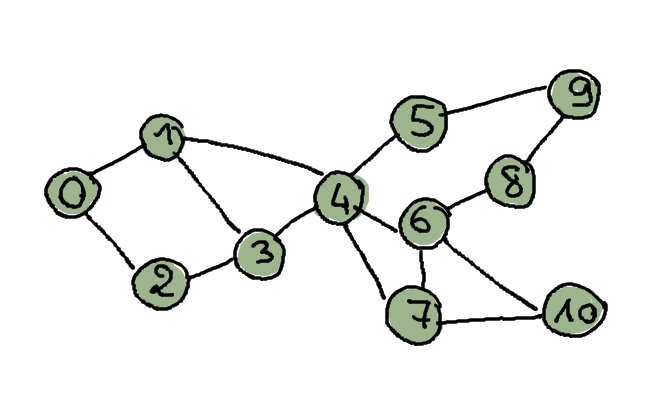
\includegraphics[width=0.6\textwidth]{Pictures/SP/shortest_path_graph.png}
\end{figure}
\begin{enumerate}[(a)]
    \item Finde den küzesten Pfad zwischen \textbf{0} und \textbf{9}. Benutze einen Breitensuche-ähnlichen Verfahren.
    \item Was würdest du machen, wenn du jetzt den kürzesten Pfad zwischen \textbf{0} und \textbf{10} finden müsstest? Kannst du etwas aus der vorherigen Teilaufgabe wiederverwenden?
    \item Wie würdest du den kürzesten Pfad zwischen \textbf{6} und \textbf{0} finden? Kannst du etwas aus den vorherigen Teilaufgaben wiederverwenden?
    \item Und wenn du den kürzesten Pfad zwischen \textbf{9} und \textbf{1} finden musst?
\end{enumerate}{}
\end{aufgabe}

\begin{aufgabe}\label{aufgabe_shortest_path_alg}
Überlege wie du den Breitensuchealgorithmus verändern musst, um den kürzesten Pfad zwischen zwei Knoten zu finden. Du kannst deine Erkenntnisse aus Aufgabe \ref{aufgabe_find_shortest_path} benutzen.

Welche zusätzliche Informationen musst du speichern? Wo würdest du es machen?
Wie verwendest du diese zusätzliche Informationen, um den Pfad zu finden?

Schreibe deinen Algorithmus möglichst genau auf.
\end{aufgabe}



\subsubsection*{Der kürzeste Pfad in Python}
Wir werden jetzt zusammen eine mögliche Lösung zur Aufgabe \ref{aufgabe_shortest_path_alg} in Python implementieren. Die zwei wichtigen Unterschiede zum ersten Breitensucheprogramm haben mit den roten Pfeilen aus Abbildung \ref{fig:norbert_klein_graph_arrows} zu tun:
\begin{enumerate}
    \item Wie wir die ''rote Pfeile'' speichern
    \item Wie wir die ''rote Pfeile'' zurückverfolgen
\end{enumerate}

Zuerst werden wir das erste Breitensucheprogramm so verändern, dass wir uns für jeden besuchten Knoten merken, woher wir diesen Knoten gefunden haben. Das Programm erwartet einen Graphen und einen Startknoten und gibt für jeden erreichbaren Knoten aus, woher wir diesen Knoten gefunden haben.

\begin{lstlisting}[language=Python, caption={Programm, welches die ''rote Pfeile'' ausgehend von einem Startknoten berechnet und ausgibt. Die einzigen zwei Zeilen, die sich verändert haben, sind 3 und 10.}, label={bfs_with_parent}]
def bfs_with_parent(graph, initial):
    queue = [initial]
    visited = {initial:None}
    while queue:
        node = queue.pop(0)
        neighbours = graph[node]
        for neighbour in neighbours:
            if neighbour not in visited:
                queue.append(neighbour)
                visited[neighbour] = node
    return visited
\end{lstlisting}
Verändert haben sich die Zeilen 3 und 10. Beobachte, dass wir für die besuchten Knoten keinen Vektor mehr brauchen, sondern ein assoziatives Datenfeld, welches jedem Knoten seinen Elternknoten (das nicht spitze Ende vom ''roten Pfeil'') zuordnet. In der dritten Zeile ordnen wir dem Startknoten den speziellen Wert \texttt{None} zu, um zu signalisieren, dass er keinen Elternknoten hat. In der zehnten Zeile ordnen wir jedem neuen unbesuchten Nachbarn seinen Elternknoten zu.

Führe das Programm auf den Graphen aus der Aufgabe \ref{aufgabe_find_shortest_path} aus. Kannst du alle ''rote Pfeile'' in der Ausgabe wieder finden?
\begin{lstlisting}[language=Python]
numbers = {0: [1, 2],
        1: [0, 3, 4],
        2: [0, 3],
        3: [1, 2, 4],
        4: [1, 3, 5, 6, 7],
        5: [4, 9],
        6: [4, 7, 8, 10],
        7: [4, 6, 10],
        8: [6, 9],
        9: [5, 8],
        10:[6, 7]}

print(bfs_with_parent(numbers, 0))
{0: None, 1: 0, 2: 0, 3: 1, 4: 1, 5: 4, 6: 4, 7: 4, 8: 6, 9: 5, 10: 6}
\end{lstlisting}

Um den kürzesten Pfad zu finden, reicht es nicht, die ''roten Pfeilen'' auszugeben. Wir müssen sie auch \textbf{zurückverfolgen}.
Jetzt schreiben wir ein Programm, \texttt{backtracking}, welches genau das macht. Das Programm erwartet ein assoziatives Datenfeld, welches jedem Knoten seinen Elternknoten zuordnet (genau wie die Ausgabe von \texttt{bfs\_with\_parent}), und einen Zielknoten, und gibt den kürzesten Pfad zurück.

\begin{lstlisting}[language=Python, caption={Programm, welches ''rote Pfeile'' zurückverfolgt}, label={backtracking}]
def backtracking(parents, goal):
    reversed_path = []
    node = goal
    while node != None:
        reversed_path.append(node)
        node = parents[node]
    return list(reversed(reversed_path))
\end{lstlisting}
Das Programm fängt beim Zielknoten an und schlägt im assoziativen Datenfeld nach, woher dieser Knoten gefunden wurde. Er schlägt den Elternknoten im assoziativen Datenfeld und dessen Elternknoten und dessen Elternknoten, und es macht so weiter, bis es einen Knoten findet, der keinen Elternknoten hat. Dieser Knoten muss der Startknoten der Breitensuche gewesen sein. Mit all diesen Knoten füllt es nach und nach einen Vektor.

Beobachte, dass wir den Pfad in der letzten Zeile umdrehen müssen, sonst kriegen wir den kürzesten Pfad vom Ziel- zum Startknoten.

\begin{aufgabe}\label{aufgabe_shortest_path}
Schreibe ein Programm in Python, welches, gegeben ein Graph, ein Start- und ein Zielknoten, den kürzesten Pfad zwischen Start- und Zielknoten ausgibt. Du kannst dafür \texttt{bfs\_with\_parent} und \texttt{backtracking} verwenden.
\end{aufgabe}

\begin{framed}
\paragraph{\textcolor{blue-violet}{Was haben wir gelernt:}}
Um den \textbf{kürzesten Pfad} zwischen Start- und Zielknoten in einem Graphen zu finden, können wir eine abgeänderte Version vom Breitensuchealgorithmus verwenden. Wie in der normalen Breitensuche, verwenden wir eine Warteschlange, um die zu besuchenden Knoten zu speichern. Aber in dieser Version enthält die Warteschlange nicht nur die zu besuchende Knoten, sondern auch deren \textbf{Elternknoten}, das heisst den Knoten, wegen dem sie in die Warteschlange gelandet sind. Wir ordnen also jedem Knoten \textbf{höchstens einen} Knoten zu, als dessen Nachbar sie zur Warteschlange hinzugefügt worden sind.

Der Startknoten und jene Knoten, die vom Startknoten weiter entfernt sind als der Zielknoten, haben keinen Elternknoten.

Um den kürzesten Pfad zu finden, müssen wir die Elternknoten vom Zielknoten aus zurückverfolgen. Diesen Prozess nennt man \textbf{Backtracking}.
\end{framed}

\subsubsection*{Ein Spaziergang im All}
\begin{figure}[H]
    \centering
    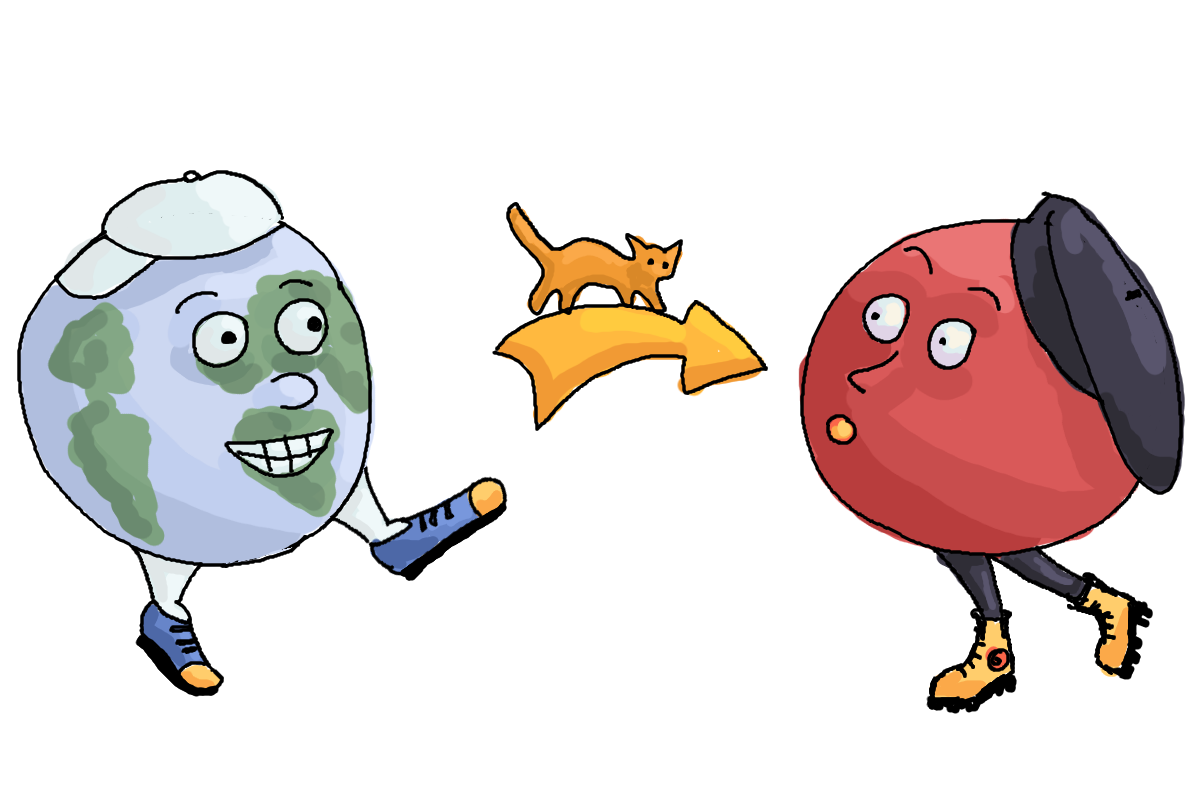
\includegraphics[width=\textwidth]{Pictures/SP/erde_mars.png}
\end{figure}
Wie weit ist es von der Erde bis zum Mars? Es kommt darauf an, wie man es misst! Wir behaupten, dass der Abstand kleiner oder gleich 12 sein muss. Und wie weit ist es von der Hand bis zum Fuss?
\begin{lstlisting}
HAND - FAND - FANS - FASS - FUSS
\end{lstlisting}
Der Sinn vom Spiel ist es eine möglichst kurze Folge von Wörter zu finden, die das Start- mit dem Zielwort verbindet, wobei alle Wörter genau 4 Buchstaben haben und zwei Wörter dürfen genau dann daneben stehen, wenn sie sich genau um einen Buchstaben unterscheiden.


\begin{aufgabe}
\begin{enumerate}[(a)]\label{aufgabe_erde_mars_graph}
    \item Formuliere das Spiel als Graph. Was sind die Knoten? Wann gibt es eine Kante zwischen zwei Knoten? Ist der Graph gerichtet oder ungerichtet?
    \item Zeichne den Graphen, der folgende Wörter modelliert:
\begin{lstlisting}
BANK, ZINS, ZANK, SINN, SAND, ZINK, SANK, ZINN
\end{lstlisting}
    \item Gibt es einen Pfad zwischen \textbf{\texttt{BANK}} und \textbf{\texttt{ZINS}}, welcher nur aus den aufgelisteten Wörter besteht?
    \item Wenn du das Wort \textbf{\texttt{ZINK}} entfenst, kannst du zwei Wörter hinzufügen, so dass \textbf{\texttt{BANK}} und \textbf{\texttt{ZINS}} immer noch verbunden sind?
\end{enumerate}

\end{aufgabe}

\begin{figure}[H]
    \centering
    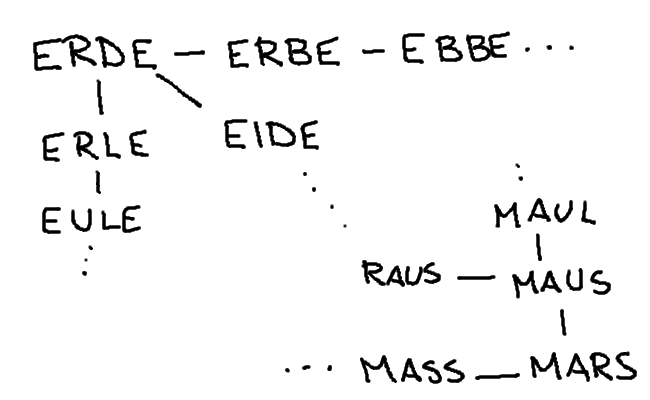
\includegraphics[width=\textwidth]{Pictures/SP/erde_mars_first_graph.png}
\end{figure}

\begin{aufgabe}\label{aufgabe_erde_mars_neighbours}
\begin{enumerate}[(a)]
    \item Schreibe den Graphen über den folgenden Wörter in der Liste der Nachbarn Darstellung.
    \begin{lstlisting}
    ERDE, EIDE, EINE, EINS, ZINS, ZINK, ZANK, ZACK, PACK, PARK, MARK, MARS,
    MAUS, HAUS, HASS, BASS, PARD, BAND, SAND, SACK, BANK, SANK, SINN, ZNINN,
    ZICK, PINS, EILT, EILE, EULE, ERLE, ENTE, ENDE
    \end{lstlisting}
    \item Rufe das Programm aus der Aufgabe \ref{aufgabe_shortest_path} auf und finde den kürzesten Pfad zwischen Erde und Mars heraus.
    \item ** Du hast bestimmt bemerkt, wie mühsam und fehleranfällig es ist, solche Graphen selber zu konstruieren und zu erweitern. Dabei ist die Idee dahinter ziemlich einfach: Nachbarwörter unterscheiden sich um einen Buchstaben. Verwende deine Kenntnisse in der Stringmanipulation und Stringkomposition, um ein Programm zu schreiben, das eine Menge von Wörter und ein Wort erwartet und alle Nachbarwörter des Wortes ausgibt, die in der Menge der Referenzwörter enthalten sind.
    \item * Schreibe das Programm aus der Aufgabe \ref{aufgabe_shortest_path} so um, dass es den Graphen nicht als Liste der Nachbarn erwartet, sondern als Liste aller Knoten, und verwende dein Programm aus der vorherigen Teilaufgabe, um die Nachbarn zu berechnen.
\end{enumerate}
\end{aufgabe}
Jetzt können wir noch mehr Wörter hinzufügen und herausfinden, was weiter von der Erde ist: der Mond oder der Mars.

\subsubsection*{\textcolor{blue-violet}{Teste dich selber}}
\begin{aufgabe}\label{pfad_kontrollfragen}
Beantworte folgende Fragen.
\begin{enumerate}[(a)]
\item Was hat die Breitensuche mit dem kürzesten Pfad zwischen zwei Knoten zu tun?
\item Welche zusätzliche Informationen muss man während der Ausführung des Breitensuchealgorithmus speichern, wenn man den kürzesten Pfad zwischen Start- und Zielknoten bestimmen möchte?
\item Was ist Backtracking? Wozu braucht man das?
\item Gregory behauptet: ''Wenn man vom Startknoten ausgehend alle Elternknoten mit dem abgeänderten Breitensuchealgorithmus findet, kann man den kürzesten Pfad zwischen dem Startknoten und allen anderen Knoten bestimmen, ohne die Breitensuche ein zweites Mal ausführen zu müssen''. Hat er recht? Begründe deine Antwort.
\item Hannah behauptet: ''Wenn man von einem Knoten ausgehend alle Elternknoten einmal berechnet hat, kann man dann den kürzesten Pfad zwischen zwei beliebigen Knoten im Graphen bestimmen, ohne die Breitensuche nochmal ausführen zu müssen.'' Hat sie recht? Begründe deine Antwort.
\end{enumerate}
\end{aufgabe}

\begin{aufgabe}\label{wikipedia_kontrollaufgabe}
Betrachte folgenden Graphen, welcher die Verlinkung von 11 Wikipediaartikeln darstellt.
\begin{figure}[H]
    \centering
    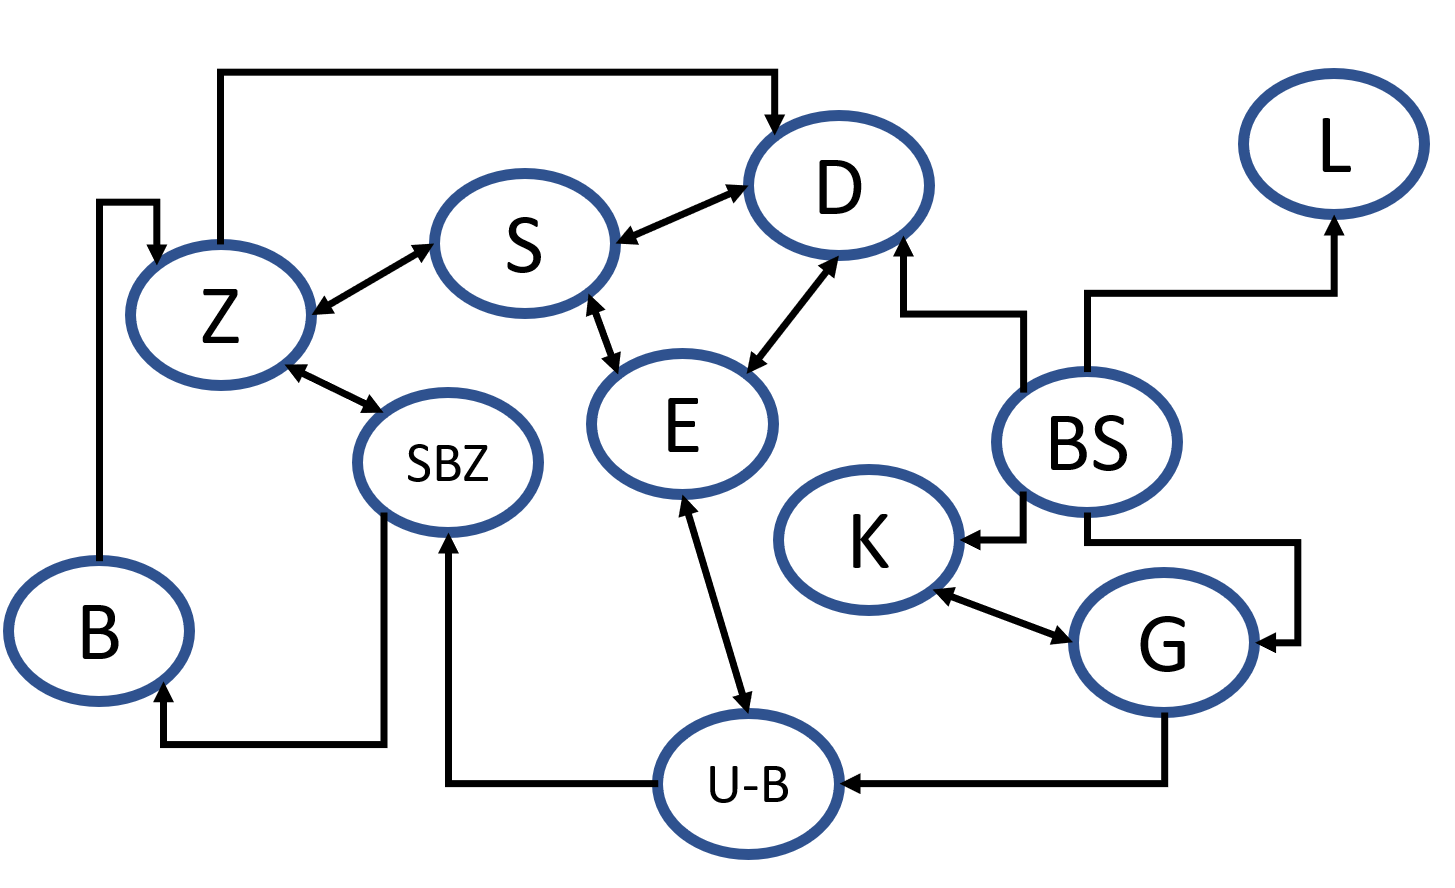
\includegraphics[width=0.7\textwidth]{Pictures/Wikipedia.PNG} 
    \caption{Die Verlinkung von Wikipediaartikeln als Graph.}
\end{figure}
\begin{enumerate}[(a)]
\item Benutze die Breitensuche, um den kürzesten Pfad zwischen \textbf{B} und \textbf{U-B} zu finden.
\item Benutze die Breitensuche, um den kürzesten Pfad zwischen \textbf{Z} und \textbf{L} zu finden.
\item Hannah behauptet: ''Wenn du \textbf{BS} als Zielknoten angibst, dann hat der Gegner keine Chance!''. Hat sie recht? Wieso?
\item Gregory behauptet: ''Um den kürzesten Pfad zwischen \textbf{B} und \textbf{D} zu finden, muss ich einfach den kürzesten Pfad zwischen \textbf{D} und \textbf{B} umdrehen.'' Stimmt das?
\item Benutze die Breitensuche, um die kürzeste Pfade zwischen \textbf{B} und \textbf{S}, zwischen \textbf{B} und \textbf{D} und zwischen \textbf{B} und \textbf{E} zu finden. Ist es einfacher, als die kürzesten Pfade zwischen \textbf{Z} und \textbf{D}, zwischen \textbf{U-B} und \textbf{D} und zwischen \textbf{SBZ} und \textbf{D} zu finden? Wieso?
\end{enumerate}
\end{aufgabe}

\paragraph{Schlangenspiel}
Alice und Bob sind zufällig in den Kinderabteil eines Zuges gelandet. Auf dem Tisch ist ein Schlangenspiel gezeichnet.
\begin{figure}[H]
    \centering
    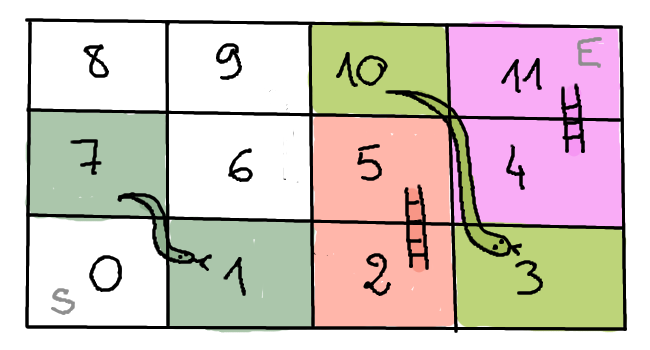
\includegraphics[width=\textwidth]{Pictures/SP/schlangen_spiel.png}
\end{figure}
Sie haben zwar keinen Würfel, aber sie verwenden zwei Münzen, um einen Würfel mit 4 Seiten zu simulieren (zum Beispiel, \texttt{(KOPF, ZAHL)} entspricht einer 1, \texttt{(ZAHL, KOPF)} einer 2, \texttt{(ZAHL, ZAHL)} einer 3 und \texttt{(KOPF, KOPF)} einer 4).
Bob will um jeden Preis gewinnen. Er hat schon herausgefunden, wie er die Resultate seiner Münzenwürfe steuert. Aber er weiss nicht, welche Zahlen rauskommen müssen, damit er mit möglichst wenig Münzenwürfe das Ziel erreicht.

\begin{aufgabe}\label{aufgabe_schlangenspiel}
\begin{enumerate}[(a)]
    \item Formalisiere das Schlangenspiel als Graph. Was sind die Knoten? Wann gibt es eine Kante zwischen zwei Knoten? Ist der Graph gerichtet oder ungerichtet?
    \item Schreibe das kleinere Spielfeld in der ''Liste der Nachbarn''-Darstellung.
    \item Was muss Bob würfeln, um zu gewinnen? Führe das Programm aus der Aufgabe \ref{aufgabe_shortest_path} aus.
    \item Schreibe das Programm aus der Aufgabe \ref{aufgabe_shortest_path} so um, dass es die Zahlen ausgibt (1, 2, 3, 4), die Bob erzielen muss.
    \item ** Überlege, was du brauchst, um die Nachbarn zu berechnen. Schreibe ein Programm, welches alle Nachbarn von einem Knoten ausgibt.
    \item * Kombiniere deine Programme aus den vorherigen Teilaufgaben und helfe Bob das Schlangenspiel auf dem grossen Spielfeld zu gewinnen. Was muss er würfeln?
    \begin{figure}[H]
    \centering
    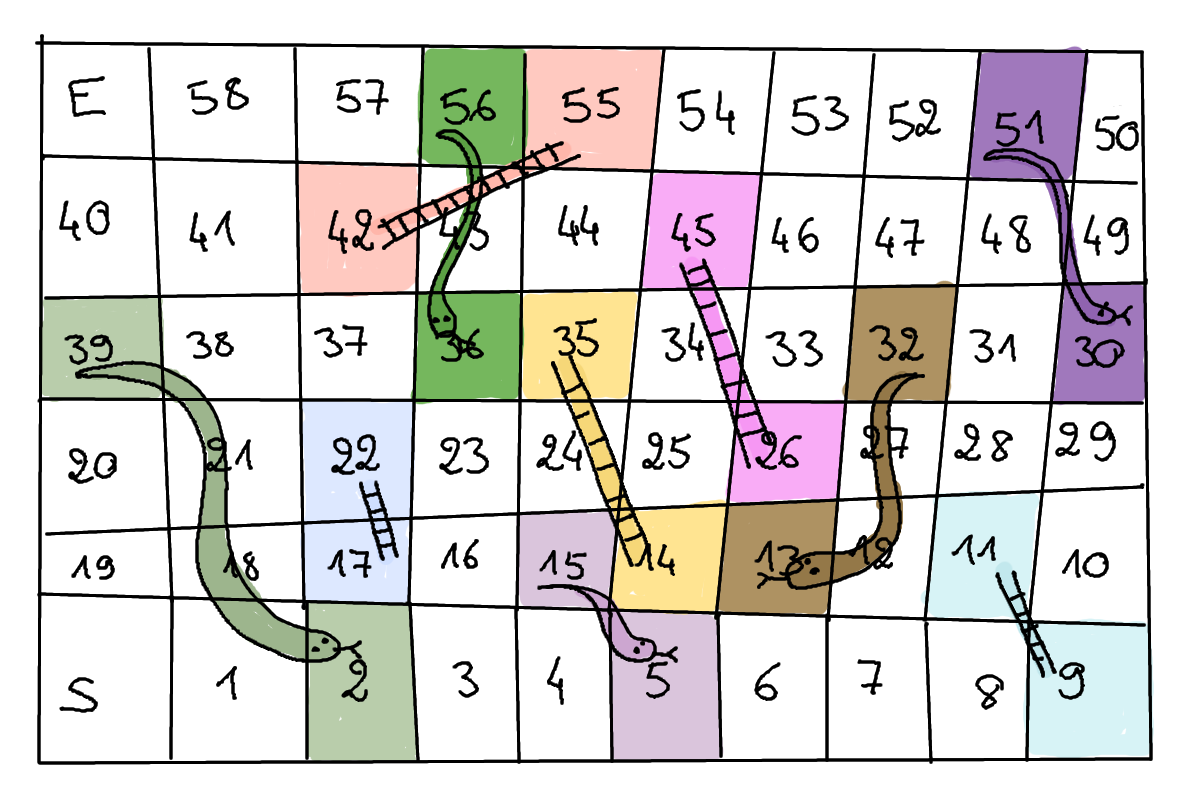
\includegraphics[width=\textwidth]{Pictures/SP/snakes_ladders_big.png}
\end{figure}
\end{enumerate}
\end{aufgabe}
